% Outfielder Recursive Loop — Real-Time Updating Cycle
% The dynamic feedback loop during active pursuit of the fly ball
% Compile with: pdflatex (requires tikz, amsmath)

\documentclass[border=12pt,tikz]{standalone}
\usepackage[T1]{fontenc}
\usepackage{amsmath}
\usepackage{tikz}
\usetikzlibrary{
  arrows.meta,
  positioning,
  calc,
  decorations.pathreplacing,
  fit,
  backgrounds,
  shapes.geometric,
  decorations.markings
}

\definecolor{actuality}{RGB}{30,60,120}
\definecolor{motion}{RGB}{140,40,40}
\definecolor{timecolor}{RGB}{60,120,60}
\definecolor{moodcolor}{RGB}{160,120,40}
\definecolor{loopcolor}{RGB}{100,100,100}
\definecolor{feedbackcolor}{RGB}{80,130,180}
\definecolor{propriocolor}{RGB}{140,80,160}
\definecolor{updatecolor}{RGB}{200,90,50}
\definecolor{perceptual}{RGB}{225,237,252}
\definecolor{cognitive}{RGB}{252,240,225}
\definecolor{actionzone}{RGB}{235,250,235}

\begin{document}
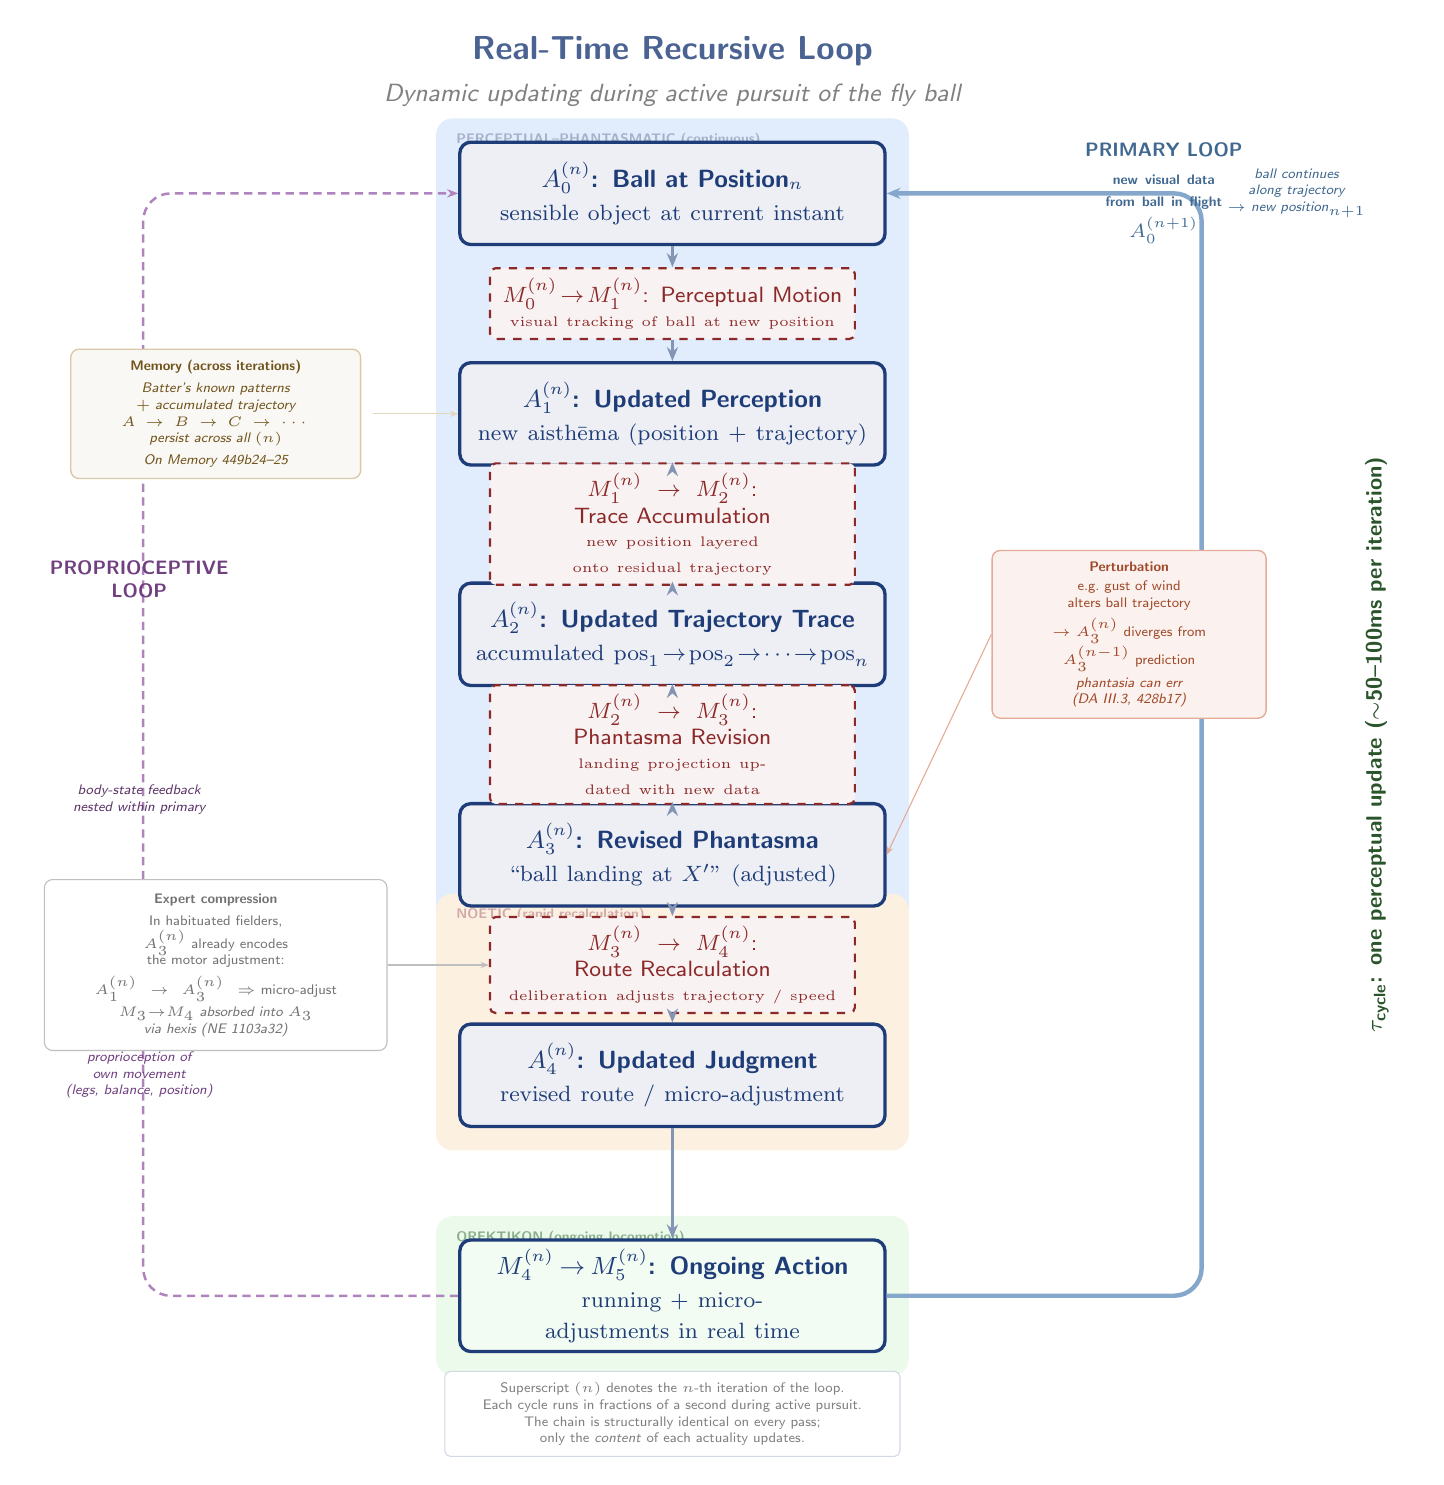
\begin{tikzpicture}[
  % --- Node styles ---
  actnode/.style={
    rectangle, rounded corners=4pt,
    draw=actuality, fill=actuality!8,
    line width=1.2pt,
    minimum width=5.4cm, minimum height=1.3cm,
    text width=5.0cm, align=center,
    font=\sffamily\small\bfseries,
    text=actuality
  },
  motionnode/.style={
    rectangle, rounded corners=2pt,
    draw=motion, fill=motion!6,
    line width=0.8pt, dashed,
    minimum width=4.6cm, minimum height=0.9cm,
    text width=4.4cm, align=center,
    font=\sffamily\footnotesize,
    text=motion
  },
  updatebox/.style={
    rectangle, rounded corners=3pt,
    draw=updatecolor!60, fill=updatecolor!6,
    line width=0.6pt,
    text width=4.0cm, align=left,
    font=\sffamily\tiny,
    text=black!65, inner sep=4pt
  },
  feedbacklabel/.style={
    font=\sffamily\tiny\itshape,
    text=feedbackcolor!80!black,
    text width=2.4cm, align=center
  },
  chainlink/.style={
    -{Stealth[length=5pt,width=4pt]},
    line width=1.2pt, color=actuality!55
  },
  feedbackarrow/.style={
    -{Stealth[length=5pt,width=4pt]},
    line width=1.2pt, color=feedbackcolor!70
  },
  proprioarrow/.style={
    -{Stealth[length=4pt,width=3pt]},
    line width=0.9pt, color=propriocolor!70, densely dashed
  },
  iterlabel/.style={
    font=\sffamily\tiny\bfseries,
    text=updatecolor!80!black,
    fill=white, fill opacity=0.9, text opacity=1,
    inner sep=2pt, rounded corners=1pt
  },
]

% ---- Layout ----
\def\nodesep{2.8}
\def\motionoff{1.4}

% ============================================================
%  PRIMARY CHAIN (center column) — one iteration cycle
% ============================================================

% Title
\node[font=\sffamily\large\bfseries, text=actuality!80]
  at (0, 1.8) {Real-Time Recursive Loop};
\node[font=\sffamily\small\itshape, text=black!50]
  at (0, 1.25) {Dynamic updating during active pursuit of the fly ball};

% -- Actualities --
\node[actnode] (A0) at (0, 0) {
  $A_0^{(n)}$: Ball at Position$_n$\\[1pt]
  {\footnotesize\normalfont sensible object at current instant}
};

\node[actnode] (A1) at (0, -\nodesep) {
  $A_1^{(n)}$: Updated Perception\\[1pt]
  {\footnotesize\normalfont new aisth\=ema (position + trajectory)}
};

\node[actnode] (A2) at (0, -2*\nodesep) {
  $A_2^{(n)}$: Updated Trajectory Trace\\[1pt]
  {\footnotesize\normalfont accumulated $\text{pos}_1 \!\to\! \text{pos}_2 \!\to\! \cdots \!\to\! \text{pos}_n$}
};

\node[actnode] (A3) at (0, -3*\nodesep) {
  $A_3^{(n)}$: Revised Phantasma\\[1pt]
  {\footnotesize\normalfont ``ball landing at $X'$'' (adjusted)}
};

\node[actnode] (A4) at (0, -4*\nodesep) {
  $A_4^{(n)}$: Updated Judgment\\[1pt]
  {\footnotesize\normalfont revised route / micro-adjustment}
};

\node[actnode, fill=actionzone!60] (A5) at (0, -5*\nodesep) {
  $M_4^{(n)} \!\to\! M_5^{(n)}$: Ongoing Action\\[1pt]
  {\footnotesize\normalfont running + micro-adjustments in real time}
};

% -- Motions --
\node[motionnode] (M01) at (0, -\motionoff) {
  $M_0^{(n)} \!\to\! M_1^{(n)}$: Perceptual Motion\\[-1pt]
  {\tiny\normalfont visual tracking of ball at new position}
};

\node[motionnode] (M12) at (0, -\nodesep - \motionoff) {
  $M_1^{(n)} \!\to\! M_2^{(n)}$: Trace Accumulation\\[-1pt]
  {\tiny\normalfont new position layered onto residual trajectory}
};

\node[motionnode] (M23) at (0, -2*\nodesep - \motionoff) {
  $M_2^{(n)} \!\to\! M_3^{(n)}$: Phantasma Revision\\[-1pt]
  {\tiny\normalfont landing projection updated with new data}
};

\node[motionnode] (M34) at (0, -3*\nodesep - \motionoff) {
  $M_3^{(n)} \!\to\! M_4^{(n)}$: Route Recalculation\\[-1pt]
  {\tiny\normalfont deliberation adjusts trajectory / speed}
};

% -- Chain arrows --
\draw[chainlink] (A0.south) -- (M01.north);
\draw[chainlink] (M01.south) -- (A1.north);
\draw[chainlink] (A1.south) -- (M12.north);
\draw[chainlink] (M12.south) -- (A2.north);
\draw[chainlink] (A2.south) -- (M23.north);
\draw[chainlink] (M23.south) -- (A3.north);
\draw[chainlink] (A3.south) -- (M34.north);
\draw[chainlink] (M34.south) -- (A4.north);
\draw[chainlink] (A4.south) -- (A5.north);

% ============================================================
%  PRIMARY FEEDBACK LOOP: A5 → new A0
%  (new sensory data from ball + world feeds back)
% ============================================================

\draw[feedbackarrow, rounded corners=10pt, line width=1.6pt]
  (A5.east) -- ++(4.0, 0) -- ++(0, 5*\nodesep) -- (A0.east)
  node[pos=0.12, right=4pt, feedbacklabel, text width=2.8cm]
  {ball continues\\along trajectory\\$\to$ new position$_{n+1}$}
  node[pos=0.5, right=5pt, font=\sffamily\scriptsize\bfseries,
    text=feedbackcolor!80!black, text width=2.4cm, align=center]
  {PRIMARY LOOP\\[2pt]{\tiny new visual data}\\{\tiny from ball in flight}\\[2pt]$A_0^{(n+1)}$};

% ============================================================
%  PROPRIOCEPTIVE LOOP: body movement → new A0
%  (fielder's own running produces sensory data)
% ============================================================

% Proprioceptive loop — draw path, then place labels manually on the vertical segment
\draw[proprioarrow, rounded corners=10pt]
  (A5.west) -- ++(-4.0, 0)
  coordinate (proprio-bl)
  -- ++(0, 5*\nodesep)
  coordinate (proprio-tl)
  -- (A0.west);

% Labels placed at absolute y-positions on the vertical segment for even spacing
\node[font=\sffamily\scriptsize\bfseries,
  text=propriocolor!80!black, text width=2.6cm, align=center]
  at ($(proprio-bl) + (-0.05, 0.65*5*\nodesep)$)
  {PROPRIOCEPTIVE\\LOOP};

\node[font=\sffamily\tiny\itshape,
  text=propriocolor!65!black, text width=2.6cm, align=center]
  at ($(proprio-bl) + (-0.05, 0.45*5*\nodesep)$)
  {body-state feedback\\nested within primary};

\node[font=\sffamily\tiny\itshape,
  text=propriocolor!80!black, text width=2.6cm, align=center]
  at ($(proprio-bl) + (-0.05, 0.2*5*\nodesep)$)
  {proprioception of\\own movement\\(legs, balance, position)};

% ============================================================
%  WIND / UNEXPECTED EVENT — perturbation injection
% ============================================================

\node[rectangle, rounded corners=3pt, draw=updatecolor!50,
  fill=updatecolor!8, line width=0.5pt,
  font=\sffamily\tiny, text=updatecolor!80!black,
  text width=3.2cm, align=center, inner sep=4pt]
  (wind) at (5.8, -2*\nodesep) {
  \textbf{Perturbation}\\[1pt]
  e.g.\ gust of wind\\
  alters ball trajectory\\[2pt]
  $\to$ $A_3^{(n)}$ diverges from\\
  $A_3^{(n-1)}$ prediction\\[2pt]
  {\itshape phantasia can err}\\
  {\itshape (DA III.3, 428b17)}
};

\draw[-{Stealth[length=3pt]}, updatecolor!50, thin]
  (wind.west) -- (A3.east);

% ============================================================
%  HEXIS COMPRESSION NOTE — expert shortcut within loop
% ============================================================

\node[rectangle, rounded corners=3pt, draw=black!25,
  fill=white, line width=0.4pt,
  font=\sffamily\tiny, text=black!55,
  text width=4.0cm, align=center, inner sep=5pt]
  (hexis) at (-5.8, -3*\nodesep - \motionoff) {
  \textbf{Expert compression}\\[2pt]
  In habituated fielders,\\
  $A_3^{(n)}$ already encodes\\
  the motor adjustment:\\[2pt]
  $A_1^{(n)} \to A_3^{(n)} \Rightarrow$ micro-adjust\\[2pt]
  {\itshape $M_3{\to}M_4$ absorbed into $A_3$}\\
  {\itshape via hexis (NE 1103a32)}
};

\draw[-{Stealth[length=3pt]}, black!25, thin]
  (hexis.east) -- (M34.west);

% ============================================================
%  ITERATION MARKERS (superscript n notation explained)
% ============================================================

\node[rectangle, rounded corners=2pt, draw=actuality!20,
  fill=white, line width=0.4pt,
  font=\sffamily\tiny, text=black!50,
  text width=5.5cm, align=center, inner sep=4pt]
  at (0, -5*\nodesep - 1.5) {
  Superscript $(n)$ denotes the $n$-th iteration of the loop.\\
  Each cycle runs in fractions of a second during active pursuit.\\
  The chain is structurally identical on every pass;\\
  only the \textit{content} of each actuality updates.
};

% ============================================================
%  BACKGROUND ZONES
% ============================================================

\begin{scope}[on background layer]
  % Perceptual-phantasmatic zone (A0–A3)
  \node[fill=perceptual, rounded corners=6pt, inner sep=8pt,
    fit=(A0)(A3)(M01)(M23),
    label={[font=\sffamily\tiny\bfseries, text=actuality!40,
      anchor=north west, xshift=4pt, yshift=-2pt]north west:
      PERCEPTUAL--PHANTASMATIC (continuous)}] {};

  % Cognitive zone (A4)
  \node[fill=cognitive, rounded corners=6pt, inner sep=8pt,
    fit=(A4)(M34),
    label={[font=\sffamily\tiny\bfseries, text=motion!40,
      anchor=north west, xshift=4pt, yshift=-2pt]north west:
      NOETIC (rapid recalculation)}] {};

  % Action zone (A5 / ongoing)
  \node[fill=actionzone, rounded corners=6pt, inner sep=8pt,
    fit=(A5),
    label={[font=\sffamily\tiny\bfseries, text=timecolor!60,
      anchor=north west, xshift=4pt, yshift=-2pt]north west:
      OREKTIKON (ongoing locomotion)}] {};
\end{scope}

% ============================================================
%  TEMPORAL ANNOTATION — cycle duration
% ============================================================

\node[timecolor!70!black, font=\sffamily\footnotesize\bfseries,
  rotate=90, anchor=south]
  at ($(A0.east) + (6.5, -2.5*\nodesep)$)
  {$\tau_{\text{cycle}}$: one perceptual update
   ($\sim$50--100ms per iteration)};

% ============================================================
%  MEMORY BACKGROUND — operates across iterations
% ============================================================

\node[rectangle, rounded corners=3pt, draw=moodcolor!40,
  fill=moodcolor!5, line width=0.5pt,
  font=\sffamily\tiny\itshape, text=moodcolor!70!black,
  text width=3.4cm, align=center, inner sep=4pt]
  at (-5.8, -\nodesep) {
  \textbf{Memory (across iterations)}\\[2pt]
  Batter's known patterns\\
  $+$ accumulated trajectory\\
  $A \!\to\! B \!\to\! C \!\to\! \cdots$\\
  persist across all $(n)$\\[2pt]
  {\tiny On Memory 449b24--25}
};

\draw[-{Stealth[length=3pt]}, moodcolor!30, thin]
  (-5.8 + 2.0, -\nodesep) -- (A1.west |- {0, -\nodesep});

\end{tikzpicture}
\end{document}
